% Adapted from SZU Experiment Report Template (Chao Fan, Kewei Ou; course 2026 edition).
\documentclass[a4paper,12pt]{article}
\usepackage{fontspec,xeCJK}
\IfFontExistsTF{Noto Serif CJK SC}{\setCJKmainfont{Noto Serif CJK SC}}{\setCJKmainfont{SimSun}[AutoFakeBold=2]}
\IfFontExistsTF{Noto Serif CJK SC}{\setCJKmonofont{Noto Serif CJK SC}}{\setCJKmonofont{SimSun}}
\usepackage[margin=1in]{geometry}
\usepackage{amsmath,booktabs,graphicx,caption,tikz,fancyhdr}
\usetikzlibrary{calc}
\renewcommand{\figurename}{图}
\renewcommand{\tablename}{表}
\captionsetup{font=small,labelfont=bf}
\setlength{\headheight}{15pt}
\setlength{\parindent}{2em}
\setlength{\parskip}{.25em}
\linespread{1.10}
\pagestyle{fancy}
\fancyhf{}
\fancyhead[L]{\small 深圳大学实验报告}
\fancyhead[R]{\small Python 程序设计 · 小项目 1}
\fancyfoot[C]{\thepage}
\newcommand{\code}[1]{\texttt{\detokenize{#1}}}
\newcommand{\field}[2]{\makebox[3.2cm][l]{\textbf{#1}}\underline{\makebox[8cm][c]{\large #2}}\\[.55cm]}
\begin{document}
\begin{titlepage}
\centering
\vspace*{2cm}
{\Huge\bfseries 深\ 圳\ 大\ 学\ 实\ 验\ 报\ 告}\\[1.5cm]
{\Large
\field{课程名称}{Python 程序设计}
\field{项目名称}{小项目 1：NumPy 图像特征提取}
\field{学\quad\quad 院}{人工智能学院}
\field{专\quad\quad 业}{人工智能（IEEE 荣誉班）}
\field{指导教师}{舒婷}
\makebox[3.2cm][l]{\textbf{报\quad 告\quad 人}}\underline{\makebox[2.5cm][c]{\large 黄锐涵}}\hspace{.4cm}\textbf{学号}\ \underline{\makebox[3.4cm][c]{\large 2025681092}}\\[.55cm]
\field{实验时间}{2026 年 11 月 9 日}
\field{提交时间}{2026 年 11 月 20 日}
}
\vfill
{\Large\bfseries 教务处制}
\end{titlepage}
\setcounter{page}{1}

\section{图像分块与多头注意力计算}
本实验用 NumPy 完成六组、共十处填空，为每张课程样例图像提取一行 512 维特征。课程提供权重、预处理和辅助函数。

\subsection{TODO-01：图像分块与像素顺序}
\textbf{过程与思考。}要让第 \(7r+c\) 行对应网格第 \(r\) 行、第 \(c\) 列的块。先把高、宽各拆成「网格坐标、块内坐标」，得到 \([B,3,7,32,7,32]\)，再用 \((0,2,4,1,3,5)\) 的轴顺序 把两个网格轴移到前面。这样展平后，块按从左到右、从上到下排列，块内按通道、行、列排列。

\textbf{核对。}单独切出首图左上 \(32\times32\) 区域并展平，与参考第一块完全相同。反过来直接 reshape 成 \([B,49,3072]\)，形状一样，第一块却有 3002 / 3072 个值不同。尺寸正确不代表索引正确。

\subsection{TODO-02：注意力头的拆分与换轴}
\textbf{过程与思考。}先把每个 token 的 768 维切成 \(12\times64\)，得到 \([B,50,12,64]\)。矩阵乘法把最后两轴当作矩阵，所以再换成 \([B,12,50,64]\)，让 batch 和 head 都留在矩阵轴之外。每个头处理同一张图的 50 个 token。

\textbf{核对。}换轴后的 \((b,h,t,d)\) 应对应原来的 \((b,t,64h+d)\)。用递增整数填满两张图的测试张量，逐头与原张量切片比较，12 个头全部一致。

\subsection{TODO-03：注意力计算与多头合并}
\textbf{过程与思考。}只交换 \(K\) 的最后两轴，再算 \(QK^\top/\sqrt{64}\)。每张图的每个头得到一张 \(50\times50\) 矩阵；一行固定一个 query，所以 softmax 沿 key 轴做，再以该行权重汇总 \(V\)。汇总后先换回 token 优先，再把 12 个头拼回 768 维，最后右乘输出权重转置并加偏置。

\textbf{核对。}分数应为 \([B,12,50,50]\)，合头后回到 \([B,50,768]\)。与 TODO-04 一起用首层参考输出检查；首层最大绝对误差为 \(7.147\times10^{-6}\)。

\newpage
\section{Transformer 特征编码与输出}

\subsection{TODO-04：残差连接与 MLP 计算}
\textbf{过程与思考。}先把注意力更新加到原始输入 \(X\)，得到 \(R\)。第二个 LayerNorm 读 \(R\)，它的结果通过线性层扩展到 3072 维，经过 GELU，再投影回 768 维。此时 MLP 计算的是对 \(R\) 的更新，因此第二条捷径也保留 \(R\)，不能改加 \(X\) 或归一化后的 \(R\)：
\[
R=X+\operatorname{MHA}(\operatorname{LN}_1(X)),\qquad
Y=R+\operatorname{MLP}(\operatorname{LN}_2(R)).
\]
\textbf{核对。}两条更新的宽度都必须回到 768；首层对照检查整块计算，末层 token 检查误差经过 12 层后是否仍在容差内。

\subsection{TODO-05：CLS 拼接与位置编码}
\textbf{过程与思考。}把每块的 3072 个值乘权重转置，投影到 768 维。先把 CLS 接到 49 个块前面，再按 token 轴加 50 行位置向量：第 0 行位置属于 CLS，第 1 行才属于第一个块。如果先按块加位置，就要额外处理位置索引的偏移。

\textbf{核对。}直接对照输入 token 参考。此时尚未进入注意力，出现差异可先查 patch 投影、CLS 顺序和位置对应，不必从最后的特征倒查。

\subsection{TODO-06：CLS 池化与特征归一化}
\textbf{过程与思考。}用 \code{tokens[:, 0, :]} 从每张图取 CLS，保留 batch 轴。对它做后置 LayerNorm，再乘 \([768,512]\) 的最终投影；普通线性层权重存为 \([out,in]\)，但这块投影已经是 \([in,out]\)，不用转置。最后按行归一化，而不是对整个 batch 求一个范数。

\textbf{核对。}最终特征必须同时满足三件事：每张图对应一行、和参考数值一致、每行范数接近 1。另用第 2、1、2 张图顺序运行命令行，输出 ID 和特征行都保持了这个顺序，重复图没有被丢掉。

\subsection{复现}
实测环境为 Windows CPU，Python 3.12.10、NumPy 2.2.6、Pillow 12.3.0。把课程包的 \code{weights/image_encoder.npz} 放到项目同名位置，在项目根目录执行：
\begin{verbatim}
python -m pip install -r requirements.txt
$env:OPENBLAS_NUM_THREADS = '4'
python check.py --stage all
python run.py --output evidence/output_tokens.npz
python report/make_effect.py
\end{verbatim}

\newpage
\section{运行效果：输入图像与实际特征}
下面两张图来自课程样例。折线取程序实际导出的对应特征行，只展示前 16 维；两行都完整保存为 512 维，横轴是特征下标，不是图像位置。

\begin{center}
\begin{minipage}{.44\linewidth}
\centering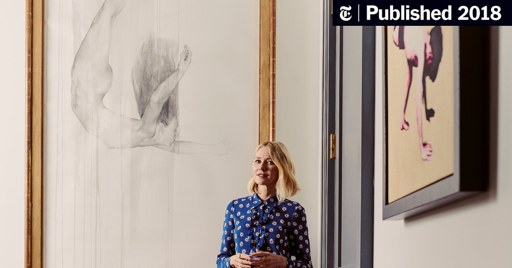
\includegraphics[width=\linewidth,height=3.25cm,keepaspectratio]{../assets/images/image_01.jpg}\\[-.15em]
{\small\ttfamily image\_01}
\end{minipage}
\begin{minipage}{.44\linewidth}
\centering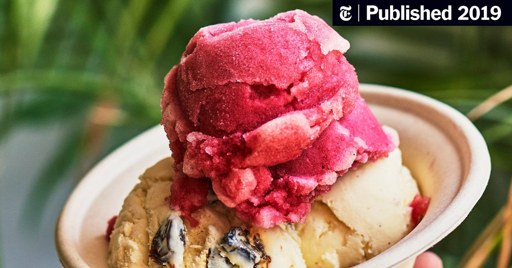
\includegraphics[width=\linewidth,height=3.25cm,keepaspectratio]{../assets/images/image_02.jpg}\\[-.15em]
{\small\ttfamily image\_02}
\end{minipage}
\par\vspace{.3em}
\begin{tikzpicture}[x=.73cm,y=1.05cm,font=\small]
\draw[gray!35] (1,-1) -- (16.25,-1);
\node[left] at (1,-1) {-0.10};
\draw[gray!35] (1,0) -- (16.25,0);
\node[left] at (1,0) {0.00};
\draw[gray!35] (1,1) -- (16.25,1);
\node[left] at (1,1) {0.10};
\draw[->] (1,-1.1) -- (1,1.28);
\draw[->] (1,-1.1) -- (16.5,-1.1);
\node[anchor=south west] at (1,1.29) {特征值};
\node[below] at (8.5,-1.55) {特征下标};
\node[below] at (1,-1.13) {1};
\node[below] at (4,-1.13) {4};
\node[below] at (8,-1.13) {8};
\node[below] at (12,-1.13) {12};
\node[below] at (16,-1.13) {16};
\draw[blue!70!black,solid,thick] plot coordinates {(1,-0.398982) (2,0.850131) (3,0.798809) (4,0.213474) (5,0.210418) (6,0.004352) (7,-0.328966) (8,0.220557) (9,-0.098742) (10,0.328150) (11,0.218835) (12,0.427833) (13,0.344998) (14,0.334128) (15,0.778881) (16,-0.345552)};
\draw[blue!70!black,solid,thick] (6,1.52) -- ++(1,0) node[right] {\ttfamily image\_01};
\draw[orange!80!black,dashed,thick] plot coordinates {(1,-0.421172) (2,-0.440907) (3,-0.246293) (4,0.379872) (5,0.254096) (6,0.104346) (7,-0.229747) (8,0.284245) (9,-0.357778) (10,0.186257) (11,0.170185) (12,0.468941) (13,-0.099706) (14,0.684479) (15,0.322179) (16,-0.557027)};
\draw[orange!80!black,dashed,thick] (11,1.52) -- ++(1,0) node[right] {\ttfamily image\_02};
\end{tikzpicture}

\end{center}

\noindent\textbf{实际导出：}\code{ids} 为 10 个图像 ID；\code{output_tokens} 为 \(10\times512\) 的 FP32 矩阵。课程检查的 8 个阶段全部通过。下表按计算顺序列出关键阶段：
\begin{center}
\small
\begin{tabular}{@{}lrr@{}}
\toprule
验证位置 & 图像数 & 最大绝对误差\\
\midrule
切块 & 2 & 0\\
输入 token & 2 & \(4.387\times10^{-5}\)\\
末层 token & 2 & \(4.196\times10^{-5}\)\\
最终特征 & 10 & \(5.662\times10^{-7}\)\\
\bottomrule
\end{tabular}
\end{center}
最终特征的最大单位范数偏差为 \(1.192\times10^{-7}\)。

\subsection{结果分析与实验反思}
直接 reshape 的反例表明，张量形状无法反映元素是否取自正确位置。遇到这类问题，可以先用一个能手工核对的小例子检查索引，再逐层比对参考输出。本次切块结果完全一致，首个非零差异出现在输入 token 阶段，因此应优先复查 patch 投影与位置向量。

两条曲线展示了特征的输出形式。逐元素对照与换序实验共同支持这 10 张样例上的数值一致性和图像对应关系。后续可增加不同宽高比的图片，核对中心裁剪，并比较同一图片单张运行和批量运行的结果。

\clearpage
\thispagestyle{empty}
\null
\begin{tikzpicture}[remember picture,overlay]
\draw[thick] ($(current page.north west)+(2cm,-3cm)$) rectangle ($(current page.south east)+(-2cm,3.5cm)$);
\node[anchor=north west] at ($(current page.north west)+(2.6cm,-3.8cm)$) {\textbf{指导教师批阅意见：}};
\node[anchor=north west] at ($(current page.north west)+(2.6cm,-12cm)$) {\textbf{成绩评定：}};
\node[anchor=north east] at ($(current page.north east)+(-2.6cm,-16cm)$) {\textbf{指导教师签字：}\hspace{2cm}};
\node[anchor=north east] at ($(current page.north east)+(-2.6cm,-17cm)$) {\textbf{年}\hspace{1cm}\textbf{月}\hspace{1cm}\textbf{日}};
\node[anchor=north west] at ($(current page.north west)+(2.6cm,-20cm)$) {\textbf{备注：}};
\node[anchor=north west,align=left,text width=16cm] at ($(current page.south west)+(2cm,3.1cm)$) {\small 注：1、报告内的项目或内容设置，可根据实际情况加以调整和补充。\\\phantom{注：}2、教师批改学生实验报告时间应在学生提交实验报告时间后 10 日内。};
\end{tikzpicture}
\vfill\null
\end{document}
